\section{Results}
\label{sec:results}
The 1M samples have been post-processed by partitioning the data set in 64 subsets, a subset for each
PDS. 
For each subset/PDS a value of probability and error estimate associated to it have been determined 
(see Section~\ref{sec:plantAnalysisResults}).

Table~\ref{tab:resultsMain} summarize these findings and range the PDS based on their probability.
First of all, note that 14 out of 64 PDSs were actually generated; i.e., none of the 1M samples 
belong to 50 PDSs.

Secondarily, note that none of the recovery strategy are able to recovery PWR3: its condition at 
the beginning of the accident is the worst among the three units (lost of CST inventory on top of 
SBO condition). From separate calculations, PWR3 could be saved only if EPE3 would be connected
withing the first 50 minutes after SBO condition. Such condition, cannot be met given the boundary
conditions of the accident progression.

PWR1, on the other side, never reach CD condition: this is due to the fact that CST inventory is 
intact (compare to PWR3) and thus time required to reach CD condition is much longer. In addition,
PWR1 can be put in safe condition through several ways (see Section~\ref{sec:testCase}).

PWR2 and the SFPs appear to reach both CD and OK condition. The objective of the analysis is now 
to understand what are the driving factors behind each PDS instead of focusing only on PDS 
probabilities. Due to the complexity of PDS8, we will leave it at the end of the analysis.

\begin{table}
  \centering
  \begin{tabular}{c|cccccc|ccc}
    \hline
    ID & \multicolumn{6}{c}{PDS} & \multicolumn{3}{c}{Probability}   \\
    \cline{2-10}
         & PWR1 & PWR2 & PWR3 & SFP1 & SFP2 & SFP3 & mean & $5^{th}$ & $95^{th}$     \\
    \hline \hline
     8    & OK   & OK   & \cellcolor[gray]{0.95}CD   & OK   & OK   & OK   & 0.890199555 & 0.889684864 & 0.890713359 \\
      12   & OK   & OK   & \cellcolor[gray]{0.95}CD   & \cellcolor[gray]{0.95}CD   & OK   & OK   & 0.058915971 & 0.058529164 & 0.059303781 \\
      10   & OK   & OK   & \cellcolor[gray]{0.95}CD   & OK   & \cellcolor[gray]{0.95}CD   & OK   & 0.033966983 & 0.033669558 & 0.034265467 \\
      9    & OK   & OK   & \cellcolor[gray]{0.95}CD   & OK   & OK   & \cellcolor[gray]{0.95}CD   & 0.012604994 & 0.012422046 & 0.012789049 \\
      24   & OK   & \cellcolor[gray]{0.95}CD   & \cellcolor[gray]{0.95}CD   & OK   & OK   & OK   & 0.002102999 & 0.002028218 & 0.002178912 \\ 
      13   & OK   & OK   & \cellcolor[gray]{0.95}CD   & \cellcolor[gray]{0.95}CD   & OK   & \cellcolor[gray]{0.95}CD   & 0.001172999 & 0.001117271 & 0.001229862 \\
      14   & OK   & OK   & \cellcolor[gray]{0.95}CD   & \cellcolor[gray]{0.95}CD   & \cellcolor[gray]{0.95}CD   & OK   & 0.000581    & 0.00054194  & 0.000621195 \\    
      11   & OK   & OK   & \cellcolor[gray]{0.95}CD   & OK   & \cellcolor[gray]{0.95}CD   & \cellcolor[gray]{0.95}CD   & 0.000165    & 0.000144457 & 0.00018668  \\     
      26   & OK   & \cellcolor[gray]{0.95}CD   & \cellcolor[gray]{0.95}CD   & OK   & \cellcolor[gray]{0.95}CD   & OK   & 0.000156    & 0.000136041 & 0.000177095 \\
      28   & OK   & \cellcolor[gray]{0.95}CD   & \cellcolor[gray]{0.95}CD   & \cellcolor[gray]{0.95}CD   & OK   & OK   & 0.000111    & 9.43E-05    & 0.000128878 \\
      25   & OK   & \cellcolor[gray]{0.95}CD   & \cellcolor[gray]{0.95}CD   & OK   & OK   & \cellcolor[gray]{0.95}CD   & 1.10E-05    & 6.17E-06    & 1.70E-05    \\ 
     15   & OK   & OK   & \cellcolor[gray]{0.95}CD   & \cellcolor[gray]{0.95}CD   & \cellcolor[gray]{0.95}CD   & \cellcolor[gray]{0.95}CD   & 6.00E-06    & 2.61E-06    & 1.05E-05    \\     
     30   & OK   & \cellcolor[gray]{0.95}CD   & \cellcolor[gray]{0.95}CD   & \cellcolor[gray]{0.95}CD   & \cellcolor[gray]{0.95}CD   & OK   & 5.00E-06    & 1.97E-06    & 9.15E-06    \\         
     29   & OK   & \cellcolor[gray]{0.95}CD   & \cellcolor[gray]{0.95}CD   & \cellcolor[gray]{0.95}CD   & OK   & \cellcolor[gray]{0.95}CD   & 1.00E-06    & 5.13E-08    & 3.00E-06    \\    
    \hline
  \end{tabular}
  \caption{Multi-unit analysis results}
  \label{tab:resultsMain}
\end{table}

PDSs number 12, 10 and 9 are characterized by a single SFP in CD condition (on top of PWR3): SFP1, 
SFP2 and SFP3 respectively. The main driver is the loss of water inventory due to the seismic induced
SFP LOCA.
This conclusion might be obvious given the nature of the system; however, if we observe the 
histogram of the recovery strategy in each of these three PDSs 
(see Fig.~\ref{fig:histPDS_12_10_9_recoveryStrategy??}) we observe a pattern.
PDS12 and PDS9 are dominated mainly by samples that follows Strategy 1 and 2 while PDS10 is 
exclusively characterized by simulations that followed Strategy 3.
This is simply due to the fact that unit prioritization allows to recover only the SFP of the unit
that has EPE connected first. Heating-up of the SFP is so fast that does not allow for two consecutive 
EPE timings to occur.

\begin{figure}
  \begin{subfigure}{.5\linewidth}
    \centering
    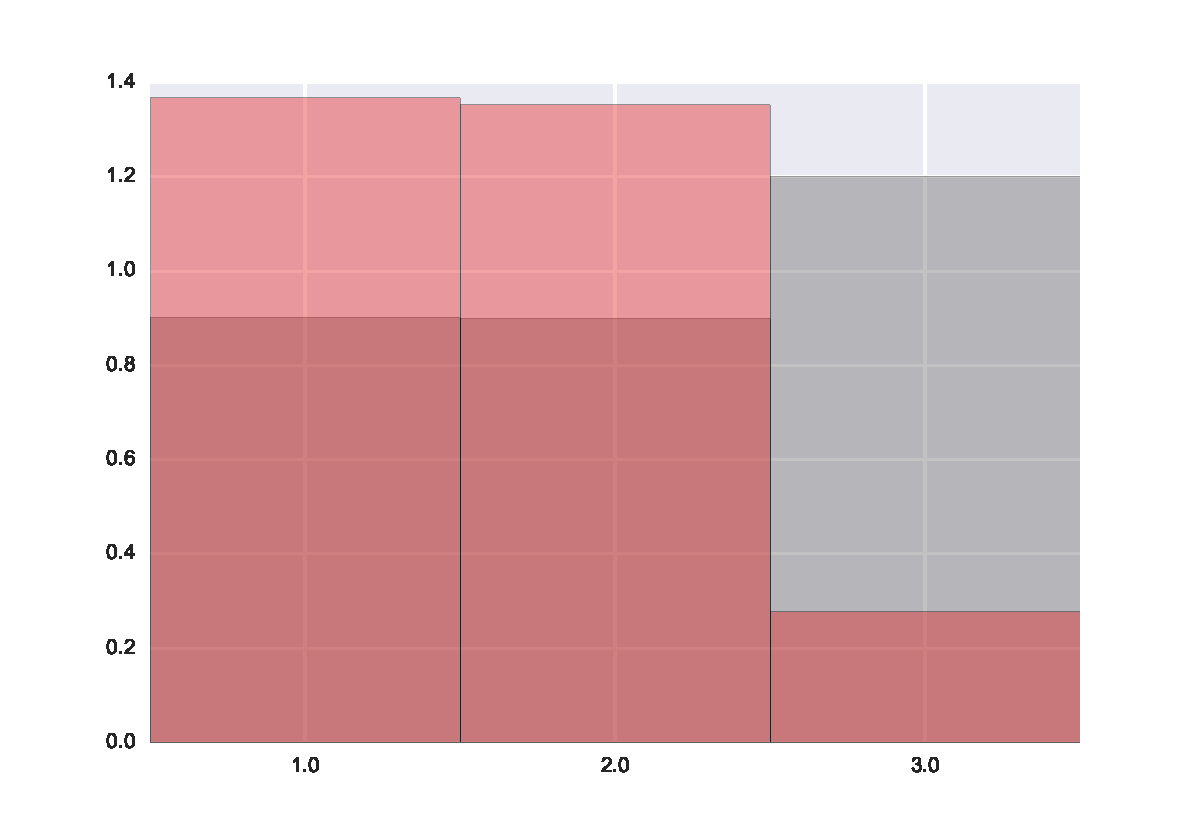
\includegraphics[scale=0.3]{12_recoveryStrategy.pdf}
  \end{subfigure}%
  \begin{subfigure}{.5\linewidth}
    \centering
    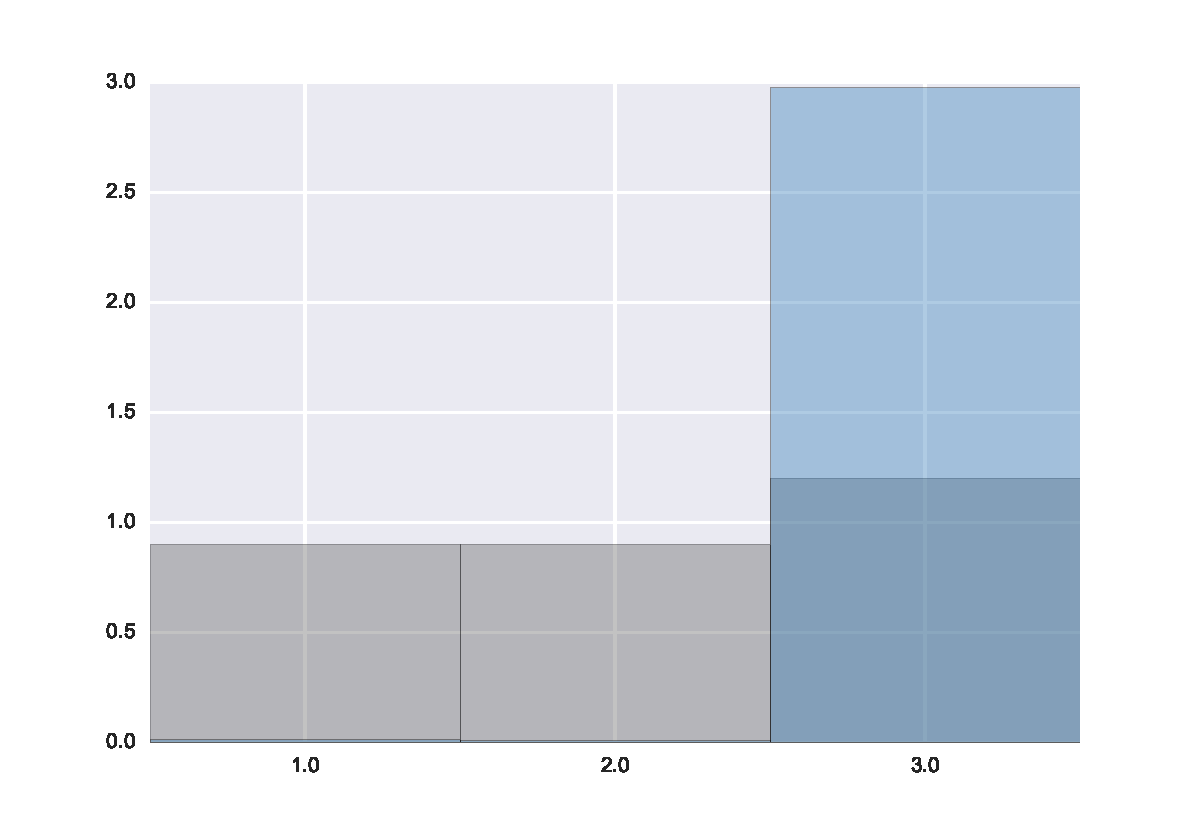
\includegraphics[scale=0.3]{10_recoveryStrategy.pdf}
  \end{subfigure}\\[1ex]
  \begin{subfigure}{\linewidth}
    \centering
    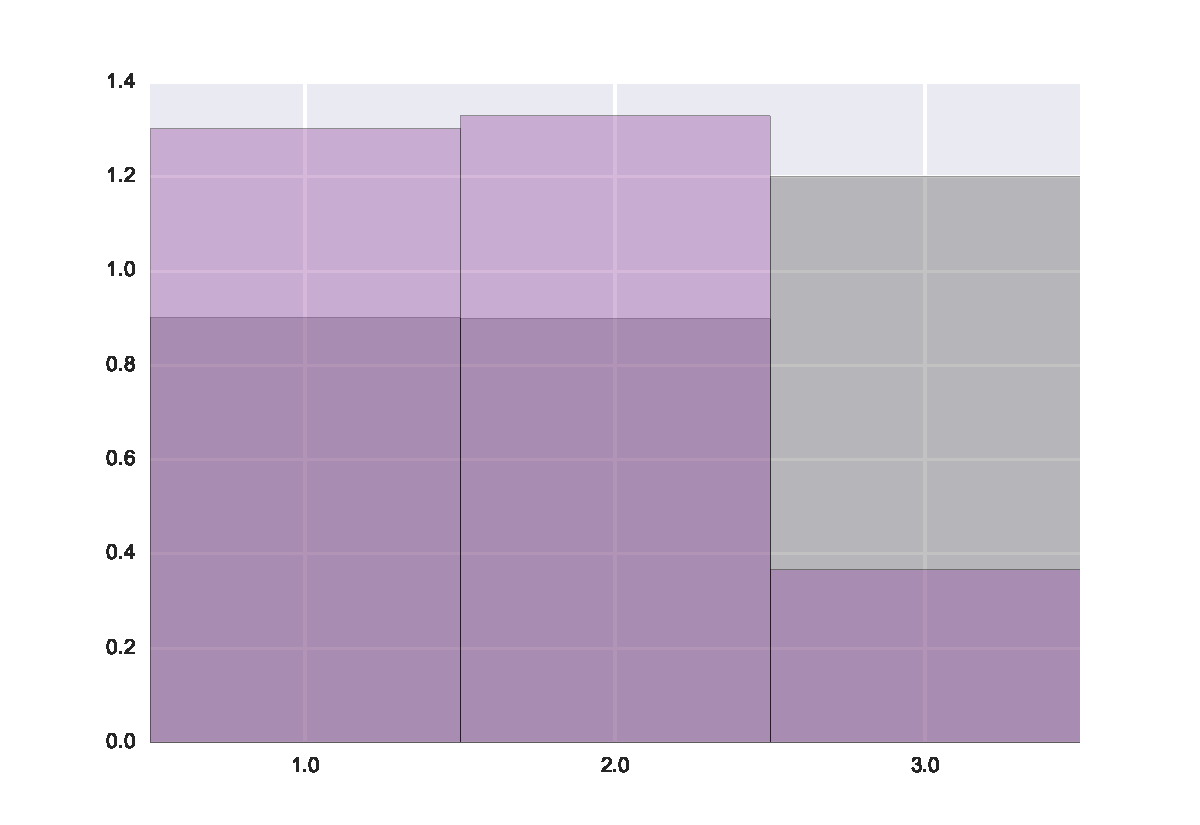
\includegraphics[scale=0.3]{9_recoveryStrategy.pdf}
  \end{subfigure}
  \caption{Histograms of the variable recovery strategy for PDS12 (top left), PDS10 (top right) and PDS9 (bottom)}
  \label{fig:histPDS_12_10_9_recoveryStrategy}
\end{figure}

PDS24 is the first PDS that characterize an additional PWR to reach CD (on top of PWR3): PWR2. By looking at the
histogram of the input parameters (see Fig.~\ref{fig:histPDS_24}) that belong to this PDS we have identified 
that PWR2 reaches CD only if recovery strategy 3 is chosen. 
In addition, involuntary alignment of EDGS plays the major driver to reach PDS24. Interestingly, the time of such 
switch is also important: by looking at bottom histogram Fig.~\ref{fig:histPDS_24}, the distribution of the 
variable EDGSinvolAlignTime is characterized by two modes, an early mode and a late mode.
This feature is due to the fact that, in strategy 3, EDGS involuntary alignment 
(see Fig.~\ref{fig:strategy3SchemeInvolAlign}) might run in parallel with EPE3 or EPE1.
If this involuntary action occurs when EPE3 or EPE1 have just started, then PWR2 reach CD almost certainly due to
the PWR2 heat-up. If this involuntary action occurs when EPE3 or EPE1 are almost completed, then the EPE team
has time to prioritize Unit 2 and quickly recovery it.
The two modes of the bottom histogram of Fig.~\ref{fig:strategy3SchemeInvolAlign} correspond to an EDGS 
involuntary action that occurs right after EPE operation for Unit 3 (early mode) and for Unit 1 (late mode) has 
started.

\begin{figure}
  \begin{subfigure}{.5\linewidth}
    \centering
    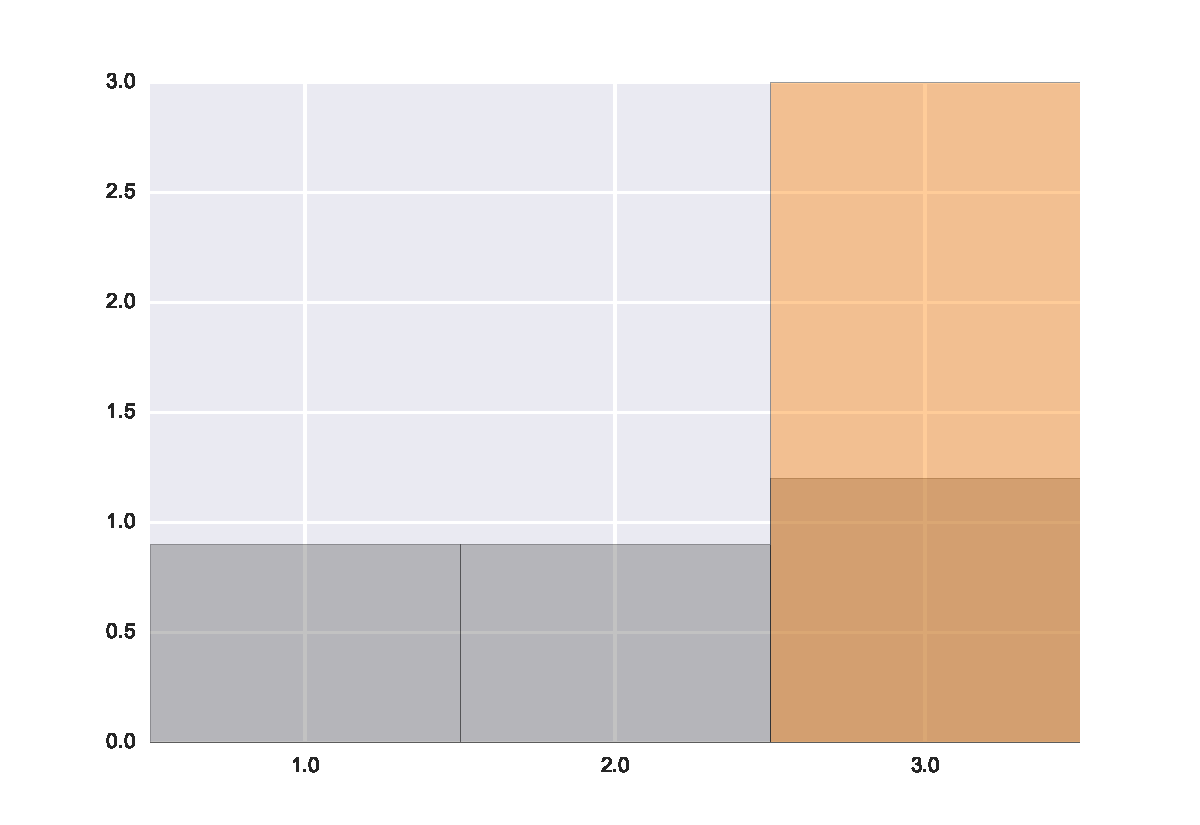
\includegraphics[scale=0.3]{24_recoveryStrategy.pdf}
  \end{subfigure}%
  \begin{subfigure}{.5\linewidth}
    \centering
    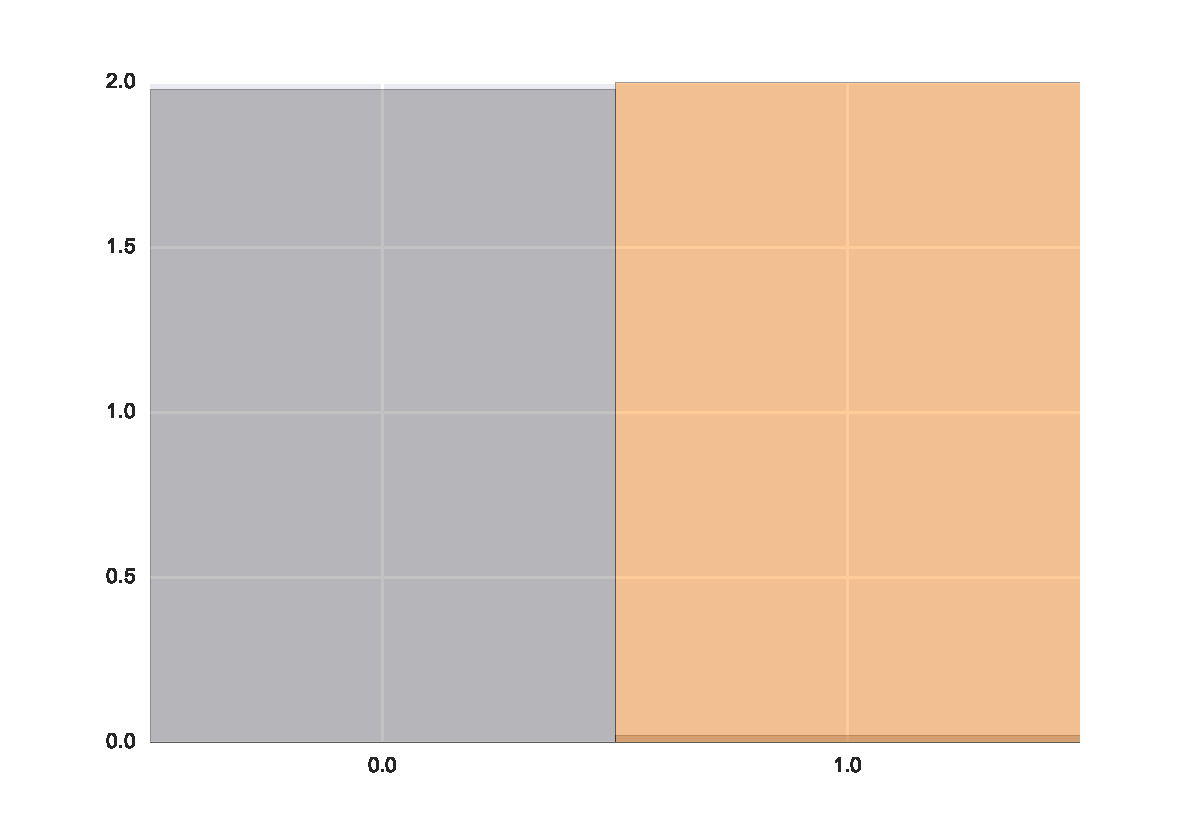
\includegraphics[scale=0.3]{24_EDGSinvolAlign.pdf}
  \end{subfigure}\\[1ex]
  \begin{subfigure}{\linewidth}
    \centering
    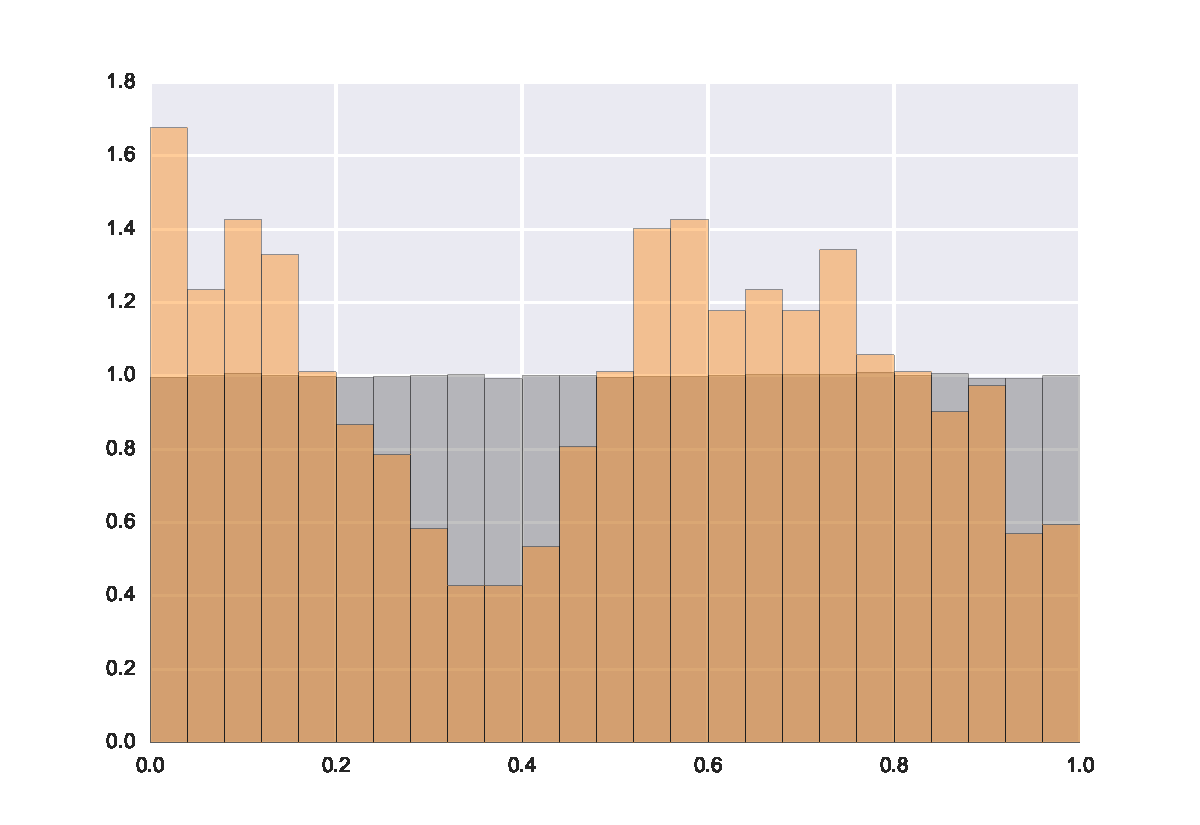
\includegraphics[scale=0.3]{24_EDGSinvolAlignTime.pdf}
  \end{subfigure}
  \caption{PDS24: histograms of the variables recovery (top left), EDGSinvolAlign (top right) and EDGSinvolAlignTime (bottom)}
  \label{fig:histPDS_24}
\end{figure}

PDSs 13, 14 and 11 is a blend of PDS 12, 10 and 9: they contains 2 SFPs in CD condition. These PDS can be simply characterized
by the occurrence of 2 SFP LOCAs which are not correlated events; i.e., SFP LOCA have been modeled as independent events.
Thus, same conclusions derived from PDSs 9, 10 and 12, can be transposed for PDSs 13, 14 and 11.

PDSs 26, 28 and 25 are characterized by 1 SFP and PWR2 in CD condition; thus it represents a mix of PDS 24 and PDS 12, 10 and 9.
These PDS are in fact characterized by recovery strategy 3 and EDGS involuntary align along with a SFP LOCA.
Similarly to what has been presented for PDS 24, the interesting histogram is the one characterized EDGS involuntary time for 
these three PDSs (see~\ref{fig:histPDS_26_28_25_EDGSinvolAlignTime}). Note these histograms follow the same pattern 
of~\label{fig:histPDS_24} (bottom plot).

\begin{figure}
  \begin{subfigure}{.5\linewidth}
    \centering
    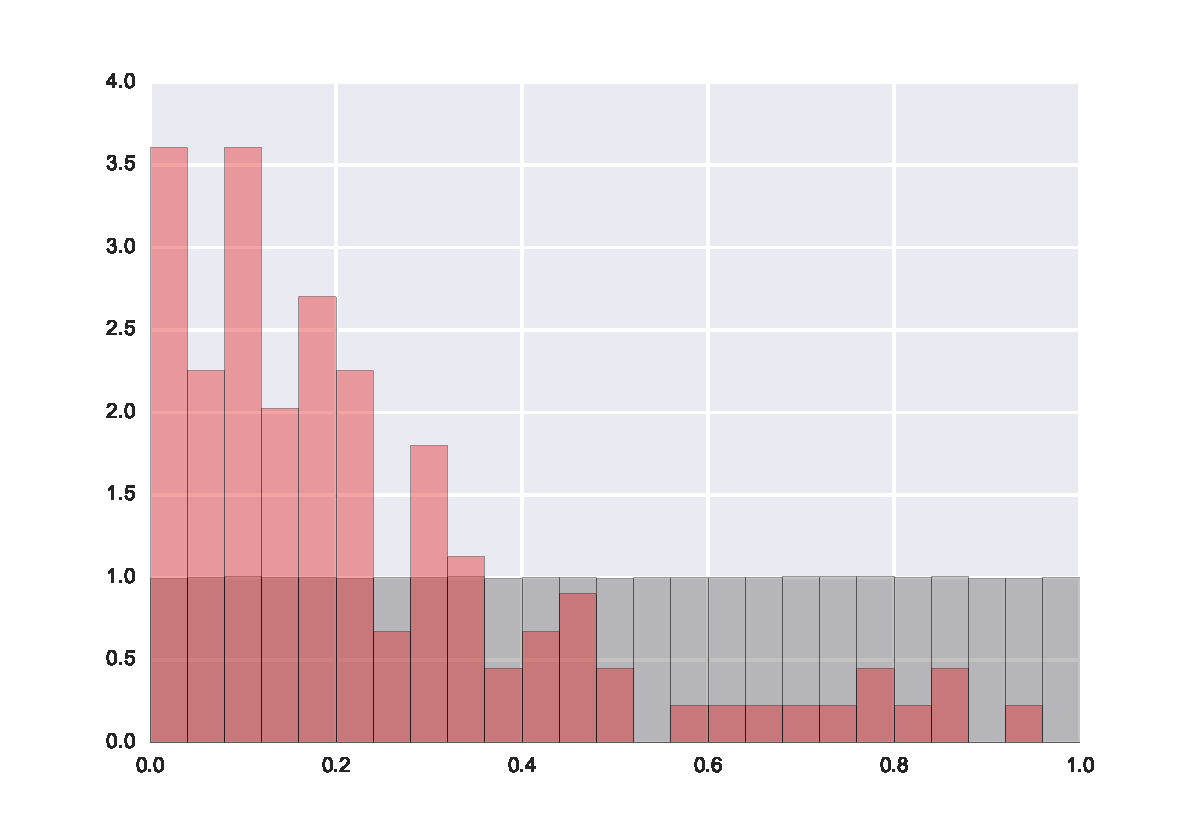
\includegraphics[scale=0.3]{28_EDGSinvolAlignTime.pdf}
  \end{subfigure}%
  \begin{subfigure}{.5\linewidth}
    \centering
    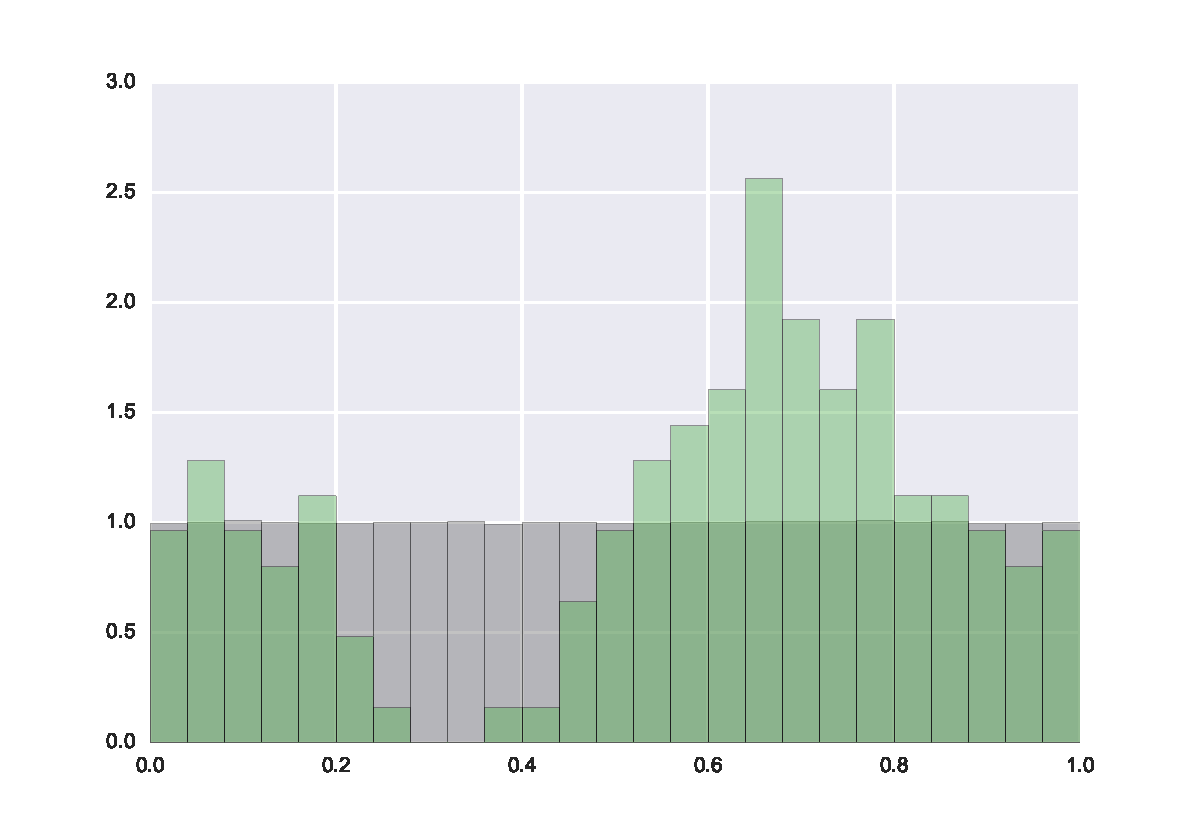
\includegraphics[scale=0.3]{26_EDGSinvolAlignTime.pdf}
  \end{subfigure}\\[1ex]
  \begin{subfigure}{\linewidth}
    \centering
    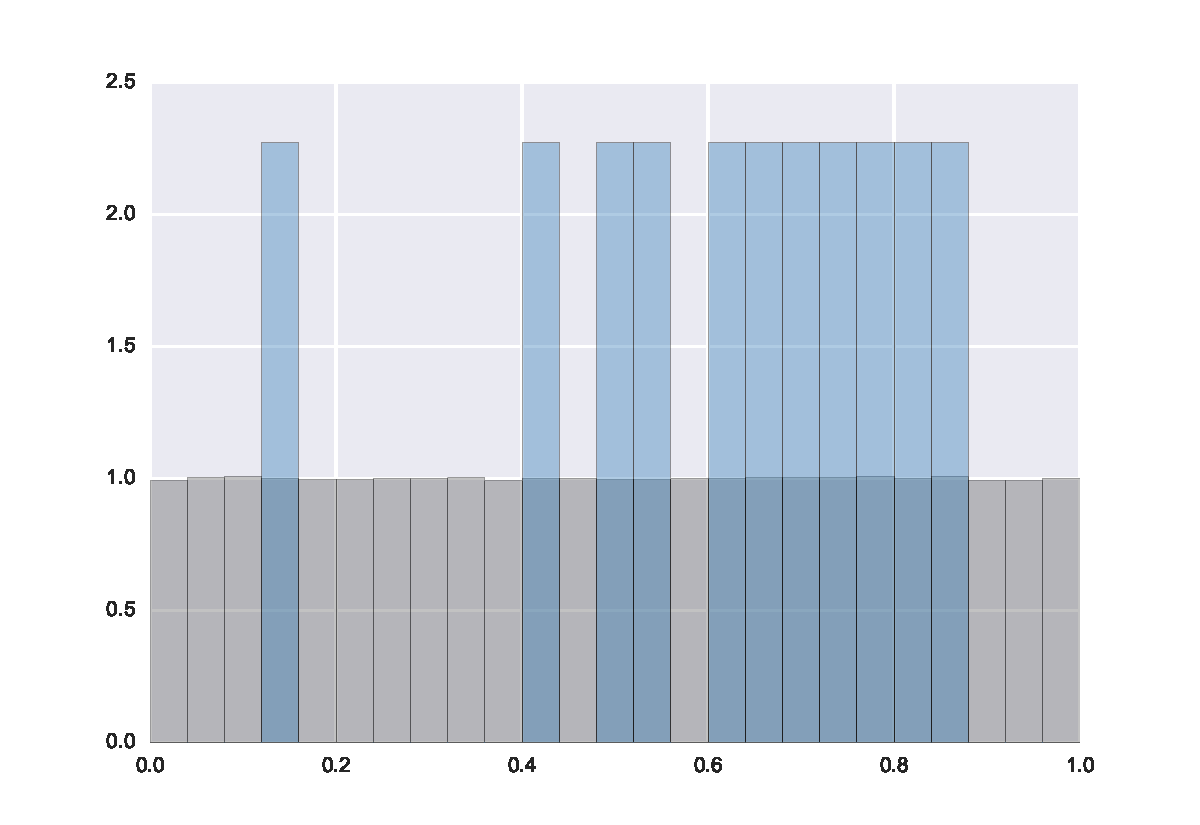
\includegraphics[scale=0.3]{25_EDGSinvolAlignTime.pdf}
  \end{subfigure}
  \caption{Histograms of the variable EDGSinvolAlignTime for PDS28 (top left), PDS26 (top right) and PDS25 (bottom)}
  \label{fig:histPDS_26_28_25_EDGSinvolAlignTime}
\end{figure}

